\subsection{Partial Order Relations}
\tsDef{3.23 (Partial Order)}{
    A \emph{partial order} on a set $A$ is a relation that is
    \emph{reflexive}, \emph{antisymmetric}, and \emph{transitive}.
    \\
    A set equipped with a partial order $\preceq$ is called a
    \emph{partially ordered set} (poset), denoted $(A,\preceq)$.
    \\
    \textbf{Examples:}
    \(
    (\mathcal{P}(A), \subseteq) \text{ is a poset},
    \)
    \(
    (\mathbb{N}_{\ge 0}, \mid) \text{ is a poset},
    \)
    \(
    (\mathbb{Z}, \preceq) \text{ is a poset}.
    \)
    \\
    Note:
    \(
    a \prec b \;\Longleftrightarrow\; a \preceq b \;\wedge\; a \ne b.
    \)
}
\newline
\tsDef{3.24 (Comparable Elements)}{
    In a poset $(A,\preceq)$, two elements $a,b \in A$ are called \emph{comparable} if
    \(
    a \preceq b \ \text{or} \ b \preceq a.
    \)
    Otherwise, they are called \emph{incomparable}.
}
\newline
\tsDef{3.25 (Total Order)}{
    Let $(A,\preceq)$ be a poset.
    If any two elements of $A$ are comparable, then $A$ is called a
    \emph{totally ordered set} (or \emph{linearly ordered}) by $\preceq$.
    \\
    \textbf{Examples:}
    \(
    (\mathbb{Z},\le) \ \text{and} \ (\mathbb{Z},\ge)
    \)
    are totally ordered,
    \((\mathcal{P}(A),\subseteq)\) is not totally ordered if $|A|\ge 2$,
    \(
    (\mathbb{N},\mid)
    \) is not totally ordered
}
\newline
\tsDef{3.26 (Covering Relation)}{
    In a poset $(A,\preceq)$, an element $b$ \emph{covers} $a$ if: \\
    \(
    a \prec b \ \text{and there is no } c \text{ with } a \prec c \prec b
    \)
    between $a$ and $b$.
}
\newline
\tsDef{3.27 (Hasse Diagram)}{
    The \emph{Hasse diagram} of a finite poset $(A,\preceq)$ is the directed graph
    whose vertices are the elements of $A$, and where there is an edge from
    $a$ to $b$ if and only if $b$ covers $a$.
    \\
    \textbf{Example:}
    \(
    (\mathcal{P}(\{a,b,c\}),\subseteq).
    \)
}
\newline
\tsDef{3.28 (Direct product of posets)}{
    Let $(A,\preceq_A)$ and $(B,\preceq_B)$ be posets.
    The direct product poset $(A\times B,\le)$ is defined by
    \(
    (a_1,b_1)\le (a_2,b_2)
    \;\Longleftrightarrow\;
    a_1 \preceq_A a_2 \;\wedge\; b_1 \preceq_B b_2.
    \)
}
\newline
\tsThe{3.12 (Direct product of posets is a poset)}{
    If $(A,\preceq_A)$ and $(B,\preceq_B)$ are posets, then
    \(
    (A,\preceq_A)\times(B,\preceq_B)
    \)
    is a partially ordered set.
}
\newline
\tsThe{3.13 (Lexicographic Order)}{
    For posets $(A,\preceq_A)$ and $(B,\preceq_B)$, the relation
    \(
    (a_1,b_1)\le_{\text{lex}}(a_2,b_2)
    \;\Longleftrightarrow\;
    a_1\prec a_2 \;\vee\; (a_1=a_2 \wedge b_1\preceq_B b_2)
    \)
    defines a partial order on $A\times B$. It is called the lexicographic order.
}
\newline
\tsDef{3.29 (Bounds)}{
    Let $(A,\preceq)$ be a poset and $S\subseteq A$. For $a\in A$:
    $\tsPoint$ $a$ is \emph{minimal / maximal} if there is no $b\in A$
    with $b\prec a$ / $b\succ a$.
    $\tsPoint$ $a$ is the \emph{least / greatest element} of $A$ if
    \(
    a\preceq b \ / \ a\succeq b \ \forall b\in A.
    \)
    $\tsPoint$ $a$ is a \emph{lower / upper bound} of $S$ if
    \(
    a\preceq b \ / \ a\succeq b \ \forall b\in S.
    \)
    $\tsPoint$ $a$ is the \emph{greatest lower bound} /
    \emph{least upper bound} of $S$ if it is respectively the
    greatest / least among all lower / upper bounds of $S$.
}
\newline
\tsDef{3.30 (Well-Ordered Set)}{
    A poset $(A,\preceq)$ is \emph{well-ordered} if it is totally ordered and
    every nonempty subset of $A$ has a least element.
    \(\tsPoint\) Every subset of a well-ordered set is also well-ordered.
}
\newline
\tsDef{3.31 (Meet and Join)}{
    Let $(A,\preceq)$ be a poset and $a,b\in A$.
    \(\tsPoint\) If $a$ and $b$ have a greatest lower bound, it is called the
    \emph{meet} and denoted $a\wedge b$.
    \(\tsPoint\) If $a$ and $b$ have a least upper bound, it is called the
    \emph{join} and denoted $a\vee b$.
}
\newline
\tsDef{3.32 (Lattice)}{
    A poset $(A,\preceq)$ in which every pair of elements has both a meet and a
    join is called a \emph{lattice}.
}
\vspace{-1.5\baselineskip}
\begin{center}
    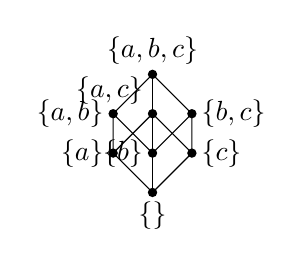
\begin{tikzpicture}[
            dot/.style={circle, fill=black, inner sep=1.2pt},
            lab/.style={font=\bfseries}
        ]

        % coordinates
        \coordinate (top) at (0,1.5);
        \coordinate (ab)  at (-0.5,1);
        \coordinate (ac)  at (0,1);
        \coordinate (bc)  at (0.5,1);

        \coordinate (a)   at (-0.5,0.5);
        \coordinate (b)   at (0,0.5);
        \coordinate (c)   at (0.5,0.5);

        \coordinate (bot) at (0,0);

        % edges (cover relations)
        \draw (top) -- (ab) -- (a) -- (bot);
        \draw (top) -- (bc) -- (c) -- (bot);
        \draw (top) -- (ac) -- (b) -- (bot);

        \draw (ab) -- (b);
        \draw (ac) -- (a);
        \draw (ac) -- (c);
        \draw (bc) -- (b);

        % dots
        \node[dot] at (top) {};
        \node[dot] at (ab)  {};
        \node[dot] at (ac)  {};
        \node[dot] at (bc)  {};
        \node[dot] at (a)   {};
        \node[dot] at (b)   {};
        \node[dot] at (c)   {};
        \node[dot] at (bot) {};

        % labels
        \node[lab, above]      at (top) {$\{a,b,c\}$};

        \node[lab, left]       at (ab)  {$\{a,b\}$};
        \node[lab, above left] at (ac)  {$\{a,c\}$};
        \node[lab, right]      at (bc)  {$\{b,c\}$};

        \node[lab, left]       at (a)   {$\{a\}$};
        \node[lab, left]      at (b)   {$\{b\}$};
        \node[lab, right]      at (c)   {$\{c\}$};

        \node[lab, below]      at (bot) {$\{\}$};
    \end{tikzpicture}
    \vspace{-0.7\baselineskip}
    \captionof{figure}{
        Lattice of the poset $(\mathcal{P}(S), \subseteq)$.
        \\
        Minimal, Least: \(\{\}\), Maximal, Greatest: \(\{\{a,b,c\}\}\).
    }
\end{center}